\documentclass[hidelinks]{article}
\usepackage[utf8]{inputenc}
\usepackage[T1]{fontenc}
\usepackage[margin=1in]{geometry}
\usepackage{amsmath,caption,graphicx,hyperref,lipsum,multicol,tabularx}
\title{Analyzing Movies Using Phrase Mining}
\author{Daniel Lee \and Huilai Miao \and Yuxuan Fan}

\begin{document}
\maketitle

\begin{abstract}
Movies often capture human culture and major events over time.
\end{abstract}

\begin{multicols}{2}
\section{Introduction}
Movies often capture human culture and major events over time. We can learn from this rich source of human history through a comprehensive textual analysis of movies, i.e., movie plot summaries. Here, we propose an analysis of movie plots by extracting key phrases corresponding to discrete entities of human culture and events. Such an analysis can help us better understand change of popular topics, public attitudes, major themes, and the overall progression of human culture throughout history. This analysis is novel since we extract history from movie plots, an unconventional source, instead of relying on historical texts directly; we expect such a study to provide a unique perspective as a result. In addition, we expect such a study to be especially useful for history non-experts, as we extract key phrases that provide relevant keywords for further research by the reader.

Previous work addresses either an analysis of movie plots or the use of phrase mining for keyword extraction, but not both. Previous analyses of movies are limited as they tend to use extract n-grams using raw frequencies instead of a sophisticated phrase mining framework such as \href{https://github.com/shangjingbo1226/AutoPhrase}{AutoPhrase} \cite{DBLP:journals/corr/ShangLJRVH17}. Here, we explore a novel approach by applying phrase mining to the analysis of movies plots.

\section{Data}
Our dataset comes from the \href{http://www.cs.cmu.edu/~ark/personas/}{CMU Movie Summary Corpus} \cite{Bamman2013LearningLP} and consists of movie plot summaries extracted from Wikipedia and movie metadata extracted from Freebase. The dataset consists of around 42,000 movies from 1893 to 2014 as seen in Figure \ref{figure:number_movies_per_year_bar_chart}, a sizable dataset for our study. Table \ref{table:dataset} describes the variables of the processed dataset. Although movies can come from different countries and may be in different languages, all of the movie plot summaries are in English (as the dataset is extracted from English Wikipedia).

\begin{figure*}
\caption{Number of movies in the dataset}
\centering
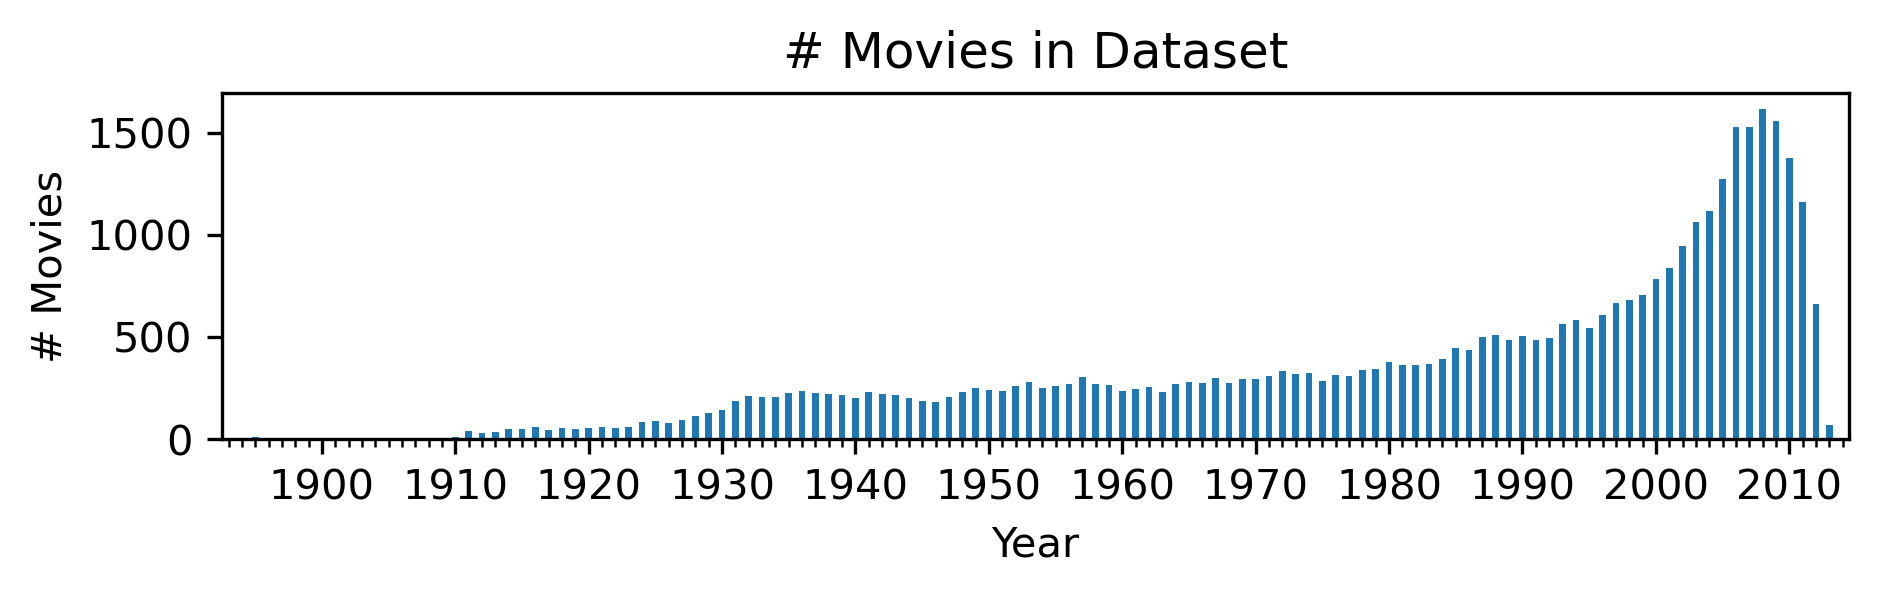
\includegraphics[width=5in]{figures/number_movies_per_year_bar_chart.png}
\label{figure:number_movies_per_year_bar_chart}
\end{figure*}

\begin{table*}
\caption{Dataset description}
\centering
\begin{tabularx}{.9\textwidth}{llX}
    \textbf{Variable} & \textbf{Description} & \textbf{Example} \\
    \hline
    name & Movie name & Star Wars Episode IV: A New Hope \\
    date & Movie release date & 1977-05-25 \\
    revenue & Movie box office revenue (USD) & 775,398,007 \\
    runtime & Movie runtime (minutes) & 122 \\
    languages & Movie languages & \{English\} \\
    countries & Movie countries & \{United States of America\} \\
    genres & Movie genres & \{Action, Adventure, Coming-of-age, Family, Fantasy, Science Fiction, Space western\} \\
    summary & Movie plot summary & The film begins with an opening crawl explaining that the galaxy is in a state of civil war and that spies for the Rebel Alliance have\ldots \\
\end{tabularx}
\label{table:dataset}
\end{table*}

\section{Methods}
Our analysis consists of three parts: exploratory data analysis (EDA), classification, and clustering.
\subsection{EDA}
Here, the tf-idf with sublinear tf scaling for a term $t$ of a document $d$ is given by
$$\text{tf-idf}(t, d) = (1 + \log\text{tf}(t, d)) \cdot \left(\log\frac{1 + n}{\text{1 + df}(t)} + 1\right)$$
where $n$ is the total number of documents and $\text{df}(t)$ is the document frequency of $t$.
\subsection{Classification}
\subsection{Clustering}

\section{Results}
\subsection{EDA}
\subsection{Classification}
\subsection{Clustering}

\section{Discussion}
\end{multicols}

\nocite{10.1145/2723372.2751523}
\bibliographystyle{plain}
\bibliography{report}

\section{Appendix}

\end{document}
